\section{Results}
\label{sec:results}
This section presents an evaluation of the results and a discussion of the model's performance, followed by an examination of the resulting trajectories from the localization pipeline. 

\subsection{SensFloor Pose Estimation Model}
The model training stopped early after 22 epochs with an overall performance of 5.5~cm MPJPE, 87\% PCK@10 and 63\% PCK@5. In the following, we visually compare an estimated to its target pose and analyze the performance across specific joints.

\subsubsection{Visual Comparison of Estimated and Target Pose} Figure \ref{fig:pose-comparison} illustrates a visual comparison between the estimated pose and the corresponding ground-truth from the test set, shown from four perspectives rotated at 0°, 90°, 180° and 270° angles. Overall, the estimated pose captures the global body posture of the target well. In particular, the global orientation of the skeleton and the left-leg joint positions align closely with the ground-truth. However, discrepancies are visible in the right lower leg, which appears shifted further back relative to the ground-truth. Furthermore, the estimated upper body exhibits a slightly stronger forward lean than the reference.

\begin{figure}[htbp] 
    \centering
    \includegraphics[width=\columnwidth]{img/pose_comparison.pdf}
    \caption{Comparison of a single estimated 3D pose (red) to its corresponding ground-truth pose (black) from four different perspectives.}
    \Description{}
    \label{fig:pose-comparison}
\end{figure}

\subsubsection{Joint Estimations}
Our recorded metrics for the test set, illustrated in Figure \ref{fig:mpjpe}, mirror the results of the visual comparison. The hip was the easiest joint to estimate with about 2~cm median error, because in the poses' local coordinate system, they mostly rotate proximal around the origin and do not move a lot.
In contrast, the wrists and ankles as the most distal joints, move the most and performed the worst, with a median of approximately 5~cm and 7~cm and a bigger interquartile range (IQR). If the model always predicted the mean pose, the overall error of all test-targets would be around 22~cm for wrists and 18~cm for the ankles. Compared to this baseline, this is a significant improvement.  

\begin{figure}[htbp]
    \centering
    \includegraphics[width=\columnwidth]{img/test_metrics_boxplot.pdf}
    \caption{Boxplot of Mean Per Joint Position Error (MPJPE) for each joint on test. The box indicates the interquartile range and the whiskers mark the $5^{th}$ and $95^{th}$ percentile.} %TODO: remove samples if not enough space
    \Description{}
    \label{fig:mpjpe}
\end{figure}

Though, while most of the data has a reasonable error, there is a significant portion with higher errors. We explained this for two reasons: First, when the subject performs an unforeseen action by rapidly changing the directions or moving their body unnaturally for example by looking at their watch, the model is not able to predict this.
Second, when the subject has just entered the SensFloor, there is no history information available and the model guesses the stepping foot. Empirical tests during inference confirmed these sources of error.

Furthermore, the ankles exhibit a significantly higher error than the elbows and wrists. This finding is counterintuitive, as the proximity of the ankles to the floor would suggest a higher localization accuracy for these joints. A potential explanation for this may lie in the target pose extraction. MediaPipe tends to estimate the same bone lengths across subjects of varying heights. These fixed proportions may lead to a misalignment between the SensFloor signals and the corresponding joint coordinates, which most significantly impacts the joints close to the floor.


\subsection{Localization and Kalman-Filter Effect}
In \ref{subsec:localization}, we introduced our approach for extracting information about the person's current global position from the SensFloor activation signals. The left side of Figure \ref{fig:kalman-filter-effect} shows the raw clustering position trajectory we recorded during a test walk. The illustrated trajectory is highly erratic. This instability is caused by two main factors. First, the algorithm creates jumps in the estimated position as the mean shifts abruptly whenever a foot makes or breaks contact with the floor. Second, the SensFloor fields produce significant background noise, even in areas where no activity takes place. While increasing the noise signal threshold suppresses some of the noise, it is not a universal solution, as signal intensity of people moving on the floor varies depending on the person's footwear. 

However, applying the Kalman filter largely reduces these issues, as illustrated on the right side of Figure \ref{fig:kalman-filter-effect}. By smoothing out the abrupt transitions and mitigating the impact of outliers, the filter produces a smooth and, according to our empirical evaluation, accurate trajectory.

\begin{figure}[htbp]
    \centering
    \includegraphics[width=\columnwidth]{img/kalman-filter-effect.pdf}
    \caption{Comparison of raw (left) and filtered (right) localization trajectories. The arrows indicate the direction of the movement, a smaller movement results in a smaller arrow.}
    \Description{}
    \label{fig:kalman-filter-effect}
\end{figure}
% - Inference works



% - evaluation
    % - Mediapipe inconsistency
    % - Only male subjects for training
    % - No groundtruth for kalman filter
    % - test set split? No evaluation that our test and trianing set have a similar distribution
    % - Model learned to Look down
    % - Only small sequences of walking possible due to the small floor (and missing API endpoint)
    % - Very limited training set with 